\lhead{\begin{tikzpicture}[remember picture, overlay]
    \node [anchor=100,inner sep=0] (imagenIZQUIERDA) at (current page header area.north){
\includegraphics[width=18cm]{img/Encabezado.PNG}};
    \end{tikzpicture}}
    \rhead{Ángeles-Hurtado}
    \rfoot{\begin{tikzpicture}[remember picture, overlay]
    \node [anchor=140,inner sep=0] (imagenDERECHA) at (current page footer area.south){
\includegraphics[width=18cm]{img/Foot.PNG}};
    \end{tikzpicture}}
    %----------------------------------------------------------------------------------------
    \lfoot{ \thepage}
    % \renewcommand{\labelenumi}{\alph{enumi}.)} 
    %----------------------------------------------------------------------------------------
    %----------------------------------------------------------------------------------------
    %	TITLE SECTION
    %----------------------------------------------------------------------------------------
    
    \setlength{\droptitle}{-5\baselineskip} % Move the title up
    \title{\textbf{Estudio de tiempos y movimientos en el ensamble de un circuito electrónico utilizando diferentes métodos para su optimización }} % Article title
    
     \author{ 
     \textsc{ Olverpa-Pérez, Eliseo Abraham}\\ 
    %  Afiliación:
     \texttt{ Instituto Tecnológico de Querétaro } \\ 
     \texttt{Tecnológico Nacional de México } \\ 
     \texttt{ Querétaro, México }\\ 
     \texttt{ l22140900@queretaro.tecnm.mx} 
     \and 
     \textsc{Ángeles-Hurtado, Luis Alberto}\\ 
    %  Afiliación:
     \texttt{ Instituto Tecnológico de Querétaro } \\ 
     \texttt{ Tecnológico Nacional de México } \\ 
     \texttt{Querétaro, México}\\ 
     \texttt{alb3rt0.ah@gmail.com} 
    }
    
    
    %----------------------------------------------------------------------------------------
    
    % \begin{document}
    
    % Print the title
    \maketitle
    \thispagestyle{fancy}
    
    %----------------------------------------------------------------------------------------
    %	ARTICLE CONTENTS
    %----------------------------------------------------------------------------------------
    
    % \section*{Resumen}
    % \textit{Palabras clave:}
    % El resumen (ancho de página) deberá contener entre 100 y 200 palabras tipo Adobe Devangari 11 puntos.
    
    \begin{abstract}
    \noindent 
    El resumen (ancho de página) deberá contener entre 100 y 200 palabras tipo Adobe Devangari 11 puntos.
    
    \end{abstract}
    % 
    % 
    \textbf{\textit{Palabras clave}}: 
    
    %\begin{itemize}
    Optimización, estudio, movimientos, tiempos, método, circuito.
    %\end{itemize}
    %
    % \keywords{First keyword should be the corresponding to the research area according with the authors guide. Maximum of 6 keywords.}
    
    \section{Introducción}
    
     %\begin{itemize}
         El estudio de tiempos y movimientos tiene la función de determinar los tiempos estándar de cada operación de un proceso del ensamblado de un circuito electrónico, al igual analizar los movimientos realizados por el operario para llevar acabo dicha operación.
    
         Terminando el siglo XlX, Frederick Taylor realizo el estudio de tiempos relacionado a las actividades laborales. Posterior al estudio de tiempos la pareja Frank y Lilian Gilbreth comenzaron el estudio de movimientos, el cual fue complementado con el estudio de tiempos de Taylor.\cite{niebel1980ingenieria}
         
         Por otro lado el estudio de movimientos tiene por objetivo eliminar o mejorar elementos que afectan a la productividad, seguridad y calidad de la producción. El estudio de tiempos es la determinación del tiempo requerido para realizar un proceso, actividad, tarea u operación específica.\cite{parra2020analisis}
    
         El estudio descrito en este proyecto tuvo por objetivo diseñar, mejorar e integrar sistemas productivos de bienes y servicios aplicando tecnologías para su optimización, además de diseñar, implementar y mejorar los sistemas de trabajo para evaluar la productividad.
     %\end{itemize} 
     %
     %
    \begin{itemize}
    
     \item Estudio de  tiempos y movimientos:Técnica que tiene por objeto, en el ámbito del trabajo, evitar movimientos innecesarios del trabajador que sólo sirven para que el tiempo de cada operación sea mayor sus objetivos son reducir, lo más posible, el tiempo necesario para ejecutar cada trabajo.\cite{patent}
     \item Ensamble: Unir, acoplar dos o más piezas.\cite{RAE}
     \item Circuito electrónico: Consiste en una estructura de placas formadas por materiales semiconductores, materiales activos y pasivos, cuyo funcionamiento es crear un recorrido completo por el cual pueda viajar la corriente. Depende del flujo de electrones para la generación, transmisión, recepción y almacenamiento de información.\cite{thomas2007principios}
     \item Método de tiempos predeterminados: Son una colección de tiempos de movimientos básicos. Se asignan a los movimientos fundamentales y a grupos de movimientos que no es posible evaluar con precisión mediante los procedimientos normales de estudio de tiempos con cronometro. Son resultado del estudio de una muestra grande de diversas operaciones con un dispositivo de tiempos como una cámara de película o de vídeo-grabación capaz de medir elementos muy cortos. \cite{niebel1980ingenieria}
     \item Optimización: Hace referencia a buscar la mejor manera de realizar una actividad.\cite{vidalesaplicacion}
     
     \end{itemize}
    % 
    %
    %
    \section{Justificación}
    
    %\begin{itemize}
    
    El presente proyecto se enfocará a la evaluación del diseño, mejora e integración sistemas productivos de bienes y servicios utilizando tecnologías para su optimización y evaluación de la productividad. 
    
    Este trabajo permitirá implementar varios métodos como el estudio de tiempos y movimientos para la optimización y mejora del ensamble de un circuito electrónico, ofreciendo un panorama a los procesos y métodos utilizados en la industria para identificar oportunidades y tener un mejor uso de los recursos. 
    
    %\end{itemize}
    % 
    % 
    \section{Descripción del problema}
    
    %\begin{itemize}
    
    Debido a la ausencia de una media y varianza conocida, existe una falta de datos históricos que dificultan la implementación y diseño de sistemas productivos y de trabajo para la evaluación de la productividad y aplicación de tecnologías para la optimización.
    
    %\end{itemize}
    %
    %
    
    \textbf{*La incógnita científica es el elemento cuya solución incrementa el conocimiento científico.}
    % 
    % 
    \section{Fundamentación teórica}
    
    Es la parte medular y de mayor discusión, deberá ser la fundamentación de la hipótesis, por tanto se deberá señalar claramente la razón de la suposición y fundamentación de la misma. Únicamente referencias científicas.
    \begin{itemize}
        \item Se debe de retomar el tema que se planteo en la introducción, pero ahora profundizando para clarificar la incógnita científica y se pueda plantear la hipótesis.
        \item Se debe de retomar la descripción del problema, pero ahora a profundidad del (los) objeto(s) de estudio. 
        \item Se debe de profundizar en las metodologías que se ha usado para el estudio del tema.
        \item Referencias solo de artículos y libros científicos.
    \end{itemize}
    % 
    % 
    \section{Hipótesis}
    
    
    
    % 
    % 
    \section{Objetivo}
    \begin{itemize}
        \item Diseña, mejora e integra sistemas productivos de bienes y servicios aplicando tecnologías para su optimización
        \item Diseña, implementa y mejora sistemas de trabajo para evaluar la productividad
    \end{itemize}
    
    \subsection{Objetivos específicos }
    
    \begin{itemize}
    
    \item Se calculará la media desconocida y varianza desconocida para la integración de los sistemas productivos
    \item Mediante la utilización del sistema de tiempos predeterminados se generarán datos históricos, que serán usados como referencia para la evaluación de la productividad
    
    \end{itemize}
    % 
    % 
    \section{Cuerpo (Metodología, modelo matemático, etc.)}
    
     Se realizará el ensamble siguiendo el Manual de ensamble circuito electrónico ESP32-C6 para poder calcular la media y varianza desconocida, buscando generar datos históricos. 
    
     Una vez se obtengan los datos históricos se hará el análisis del ensamble por medio del MTM, que es una herramienta para la elaboración de entandares que da la posibilidad de evaluar una actividad u operación y a la vez los micro movimientos, los cuales tienen un valor en TMU (unidad de tiempo en MTM), para después ser representado en segundos, minutos y horas, por lo tanto permiten obtener un valor del tiempo de la actividad realizada por un operario.\cite{navarro2006estandarizacion}
    
    Esto facilitará la identificación de áreas de oportunidad para su optimización mediante la eliminación de movimientos o la incorporación de soportes de sujeción. 
    
     A continuación se muestra la lista de los materiales, la cantidad y el nombre de los mismos que son necesarios para el ensamble.\ref{anexo:listaDeMateriales.pdf}
     Y a continuación de esta lista se muestra el Manual de ensamble circuito electrónico ESP32-C6.\ref{anexo:manualDeEnsambleCircuitoElectrónicoESP32-C6.pdf}
    
    %\begin{itemize}
     %   \item Se debe establecer que se habrá de hacer, como, conque, y donde para obtener la información que permita probar la hipótesis.  
      %  \item Se debe desglosar de acuerdo a los objetivos específicos. 
       % \item Se debe establecer una estrategia metodológica por cada objetivo específico. De manera simplista se podría decir que se cambia el verbo en infinitivo por su respectivo adverbio.
        %\item En cada objetivo se debe describir que método, que materiales y que equipo se usará para conseguirlo.
        %\item Se deben tener referencias Figura.
    %\end{itemize}
    \subsection{Prepara tu documento}
    
    Antes de que comiences a utilizar esta plantilla, es recomendable que prepare la información que contendrá en un archivo aparte. 
    Ten preparadas tus gráficas, así como también las tablas aparte, para que sea más fácil integrarlo. 
    Se recomienda fuertemente el uso de \textbf{formato Enhanced Metafile (.emf) para imágenes y gráficas} de resolución óptima. 
    Finalmente, completa y organiza el contenido antes de darle el formato de esta plantilla. 
    
    \subsection{Acrónimos y Abreviaciones}
    
    Los acrónimos y abreviaciones deberán ser definidos únicamente la primera vez que aparecen en el texto, esto para que el lector entienda lo que significan.
    
    \subsection{Ecuaciones}
    
    Las ecuaciones son una excepción a las especificaciones prescritas de esta plantilla. 
    Deberá determinar si su ecuación debe escribirse o no utilizando la fuente Adobe Devangari. 
    Para crear ecuaciones multinivel, puede ser necesario tratar la ecuación como un gráfico e insertarla en el texto después de aplicar el estilo de la platilla.
    Las ecuaciones serán enumeradas de manera consecutiva, y el número de ecuación, entre paréntesis, se colocan al ras de la derecha, utilizando una tabulación derecha. 
    
    \begin{equation}
        \label{eq1}
        x + y = z 
    \end{equation}
    
    Es importante asegurarse de que los símbolos de la ecuación sean definidos antes o inmediatamente después de la ecuación. Utilice “(1)”, en vez de “Eq. 1” al enumerar las ecuaciones, excepto al principio de una oración: “La ecuación (\ref{eq1}) es…”
    
    \section{Resultados y discusión}
    
    Antes de comenzar a preparar tu artículo, es importante que lea primero la guía del autor, la cual incluye los temas o apartados que son necesarios para tener tu trabajo completo.
    Una vez completada la edición del texto, el documento está listo para el uso de esta plantilla. En este archivo recién creado, resalte todo el contenido e importe el archivo de texto preparado. Ahora esta listo para estilizar su documento.
    En esta sección se deben presentar todo lo obtenido de la sección 2, incluidas deducciones o efectos del desarrollo. También se podrán incluir subsecciones numeradas de la siguiente forma:
    
    \subsection{Autores y Afiliaciones}
    
    Para distinguir las afiliaciones de los autores, utilice superíndices iniciando con el número 1, 2, etc., sucesivamente, esto dependerá de la cantidad de los departamentos a los que estén afiliados los autores. En caso de que todos los autores pertenezcan a una mismo departamento e institución, utilizar sólo el superíndice 1. 
    
    \subsection{Identificar los encabezados}
    
    Se les recuerda a los autores que los encabezados deben de estar conforme los solicita la guía del autor. De ahí se puede adaptar el trabajo para que sea más fácil de entender para el lector.
    Los encabezados organizan los temas sobre una base relacional y jerárquica. Por ejemplo, el título del documento es encabezado del texto principal porque todo el material posterior se relaciona y elabora sobre este tema. 
    
    \subsection{Tablas y Figuras}
    
    \begin{enumerate}
        \item Posición de las tablas y figuras: Coloque las figuras y las tablas en la parte superior e inferior de las columnas. Evite colocarlos en medio. Las figuras y las tablas grandes pueden abarcar ambas columnas. Los títulos de las figuras deben de estar debajo de las mismas; los títulos de las tablas deben aparecer encima de ellas. Insértese las figuras y los cuadros después de citarse en el texto. Utilice la abreviatura “Fig. 1”, incluso al principio de una oración. 
    \end{enumerate}
    
    \section{Conclusiones}
    
    Se describe aquí el alcance del trabajo, logros obtenidos y perspectivas para el futuro de este. Se sugiere colocar información cuantitativa obtenida.
    
    \section{Agradecimientos}
    
    Es importante darles su debido reconocimiento a los laboratorios, instituciones, organizaciones, entre otros que han sido participes para la culminación de este trabajo. También es importante mencionar, fondos, proyectos, becas, entre otros que se le han otorgado al o los autores para realizar el trabajo de investigación. Ejemplo: “Los autores agradecen al Concejo Nacional de Ciencia y Tecnología por los recursos otorgados…”
    
    % 
    % 
    %%%%%%%%%%%%%%%%%%%%%%%%%%%%%%%%%%
    \appendix
    %%%%%%%%%%%%%%%%%%%%%%%%%%%%%%%%%%
    % 
    % 
    \centering{\section[\appendixautorefname{}]
    {APÉNDICE}}\label{anexo:listaDeMateriales.pdf}
    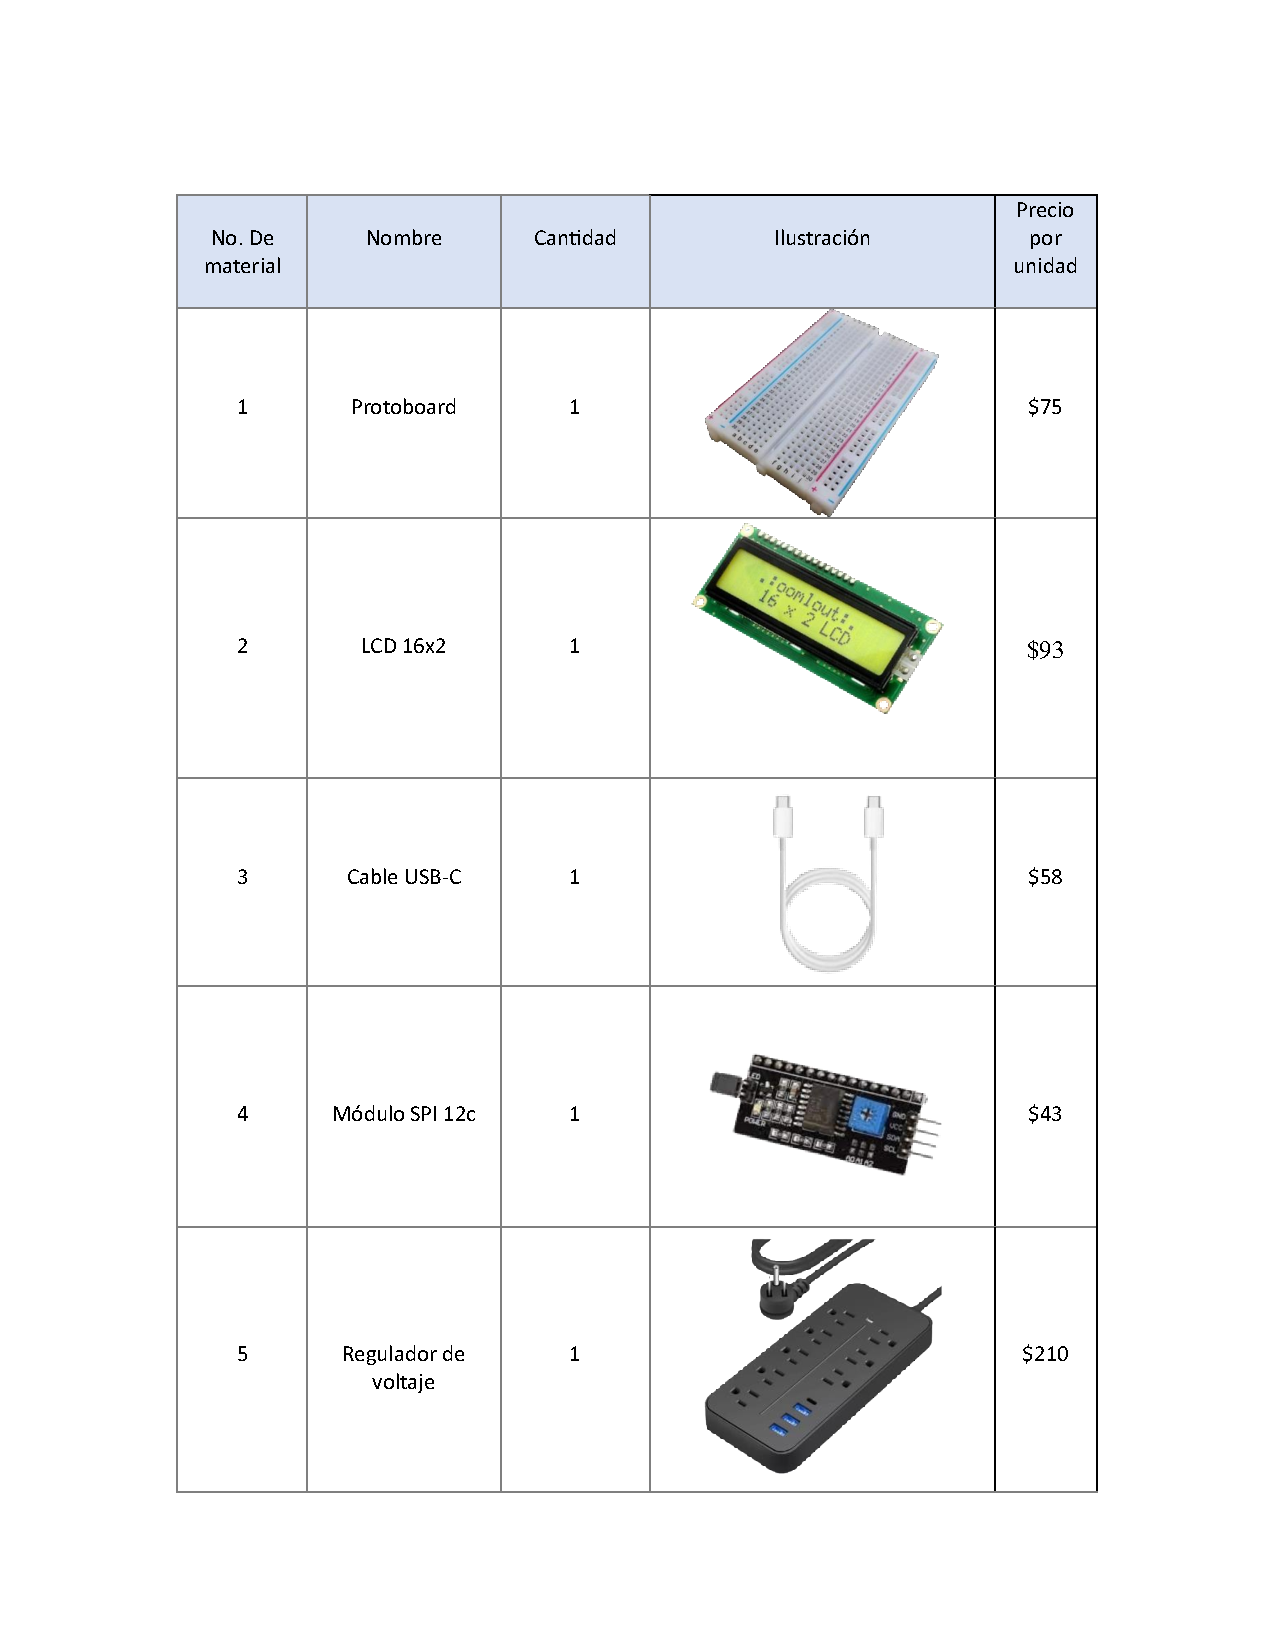
\includepdf[pages=-]{21/img/listaDeMateriales.pdf}
    %
    \centering{\section[\appendixautorefname{}]
    {APÉNDICE}}\label{anexo:manualDeEnsambleCircuitoElectrónicoESP32-C6.pdf}
    \includepdf[pages=-]{21/img/manualDeEnsambleCircuitoElectrónicoESP32-C6.pdf}
    %%%%%%%%%%%%%%%%%%%%%%%%%%%%%%%%%%%%%%%%
    \newpage
    \bibliographystyle{ieeetr}
    \bibliography{21/referencias}